\xchapter{Metodologia}{}

%O processo de mineração de opinião
%\begin{itemize}

%\item Preprocessing
%\begin{itemize}
%\item Definição
%\item Reiterar o tipo de análise escolhida: Document Level Analysis
%\item Datasets utilizados (Cornell e Amazon - descreve as caracteristicas de cada dataset, como quantidade, balanceamento, natureza, etc.)
%
%\item Descrever e justificar as tarefas envolvidas:
%\begin{itemize}
%\item O texto é dividido em sentenças
%\item POS Tagging - Brill's Tagger
%\item Blocos irrealis são filtrados ou não (atualmente NÃO FILTRAM)
%\item Defino quais ngrams serão extraídos
%\begin{itemize}
%\item Defino o uso do tipo de negação (FAR NEGATION - REFER)
%\item Os verbos foram recentemente removidos do universo
%\item Depois de testar, MANUALMENTE, diferentes configurações de n-grams, mantendo os demais parametros fixos, restaram adjetivos e adverbios, com unigrams, bigrams e trigrams
%\end{itemize}
%
%\item Retorna um vetor de n-grams (bag-of-words)
%\item Resume o subcapitulo e finaliza falando da saída dessa fase para a próxima
%\end{itemize}
%\end{itemize}
%\end{itemize}

O processo de mineração de opinião é comumente definido em seis etapas: a i) definição do domínio, ii) pré-processamento, iii) transformação, iv) seleção de características, v) classificação e vi) análise dos resultados \cite{moraes2012document}. Cada etapa inclui diferentes tarefas que, dado um documento na entrada do processo, seja possível classifica-lo e avaliar a classificação realizada.

\begin{figure}[h]
\caption{Etapas do processo de mineração de opinião.}
\centering
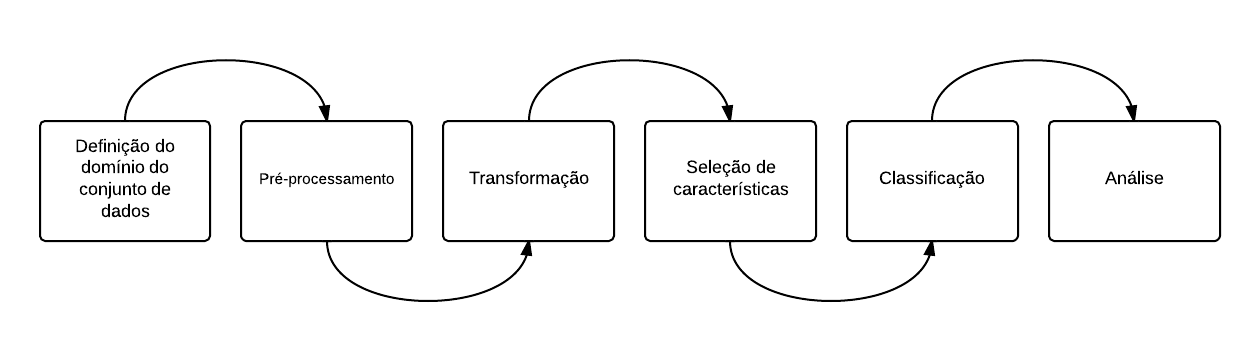
\includegraphics[scale=0.35]{opinion_mining_process.png}
\label{figura:processo_mineracao}
\end{figure}

\section{Definição do domínio e o pré-processamento dos dados}

Domínios diversos foram escolhidos para serem analisados por essa pesquisa, dentre eles filmes, livros, carros, computadores, panelas, hotéis, músicas, celulares, mp3, pen-drives, dispositivos gps, wifi e câmeras fotográficas. Essa diversidade de domínios é importante para que nós possamos corroborar nossa proposta de criar um classificador independente de domínio. Todas as bases de dados são da língua inglesa, pois os trabalhos relacionados a esta pesquisa utilizaram domínios nessa língua.

Para filmes, nós utilizamos a largamente utilizada \footnote{Vide https://www.cs.cornell.edu/people/pabo/movie-review-data/otherexperiments.html} base de dados, versão 2.0, desenvolvida e pré-classificada por \cite{pang2004sentimental}, com 2000 críticas de filmes, sendo metade positivas e outra metade negativas - bases assim, são conhecidas como balanceadas. As opiniões dos domínios de livros, carros, computadores, panelas, hotéis, músicas, celulares estão reunidos numa base de dados balanceada produzida por \cite{taboada2011lexicon}, retiradas do site Epinions \footnote{Vide http://www.epinions.com/}, com cerca de 400 críticas. E para as opiniões dos domínios de mp3, pen-drives, dispositivos gps, wifi e câmeras fotográficas, nós utilizamos uma base de dados balanceada de 2000 críticas retiradas do site da Amazon. 

Após a definição de um ou mais domínios é preciso, antes de inciar a etapa de pré-processamento, definir o nível da análise que será feita sobre os documentos. Existem três níveis básicos de análise de documentos em mineração de opinião: i) nível de análise de documento, ii) sentenças e iii) entidades e seus aspectos. O primeiro nível foca em classificar a opinião geral de um documento expressando-a como positiva ou negativa. O segundo nível, o de sentenças, em vez de considerar o sentimento geral das opiniões presentes em um documento como todo, classifica as opiniões de cada sentença separadamente. E o último nível foca em descobrir todos os alvos existentes nas sentenças do documento, e classifica as opiniões direcionadas a eles \cite{bing:2012}. Este trabalho decidiu utilizar o nível de análise de documento \cite{joachims1998text, pang2002thumbs, gamon2004sentiment, mullen2004sentiment, pang2004sentimental, cui2006comparative}.

A etapa de pré-processamento envolve tarefas como a tokenização dos documentos, marcação gramatical das palavras (do inglês, \textit{Part of Speech Tagging} ou POST), filtragem de sentenças com modais e definição os n-grams que serão utilizados para construir um modelo que represente o documento. A tokenização dos documentos é a tarefa que divide o conteúdo de cada documento em sentenças e, por sua vez, em palavras para que o marcador gramatical (ou \textit{tagger}) possa identificar as classes gramaticais das palavras do documento. O marcador gramatical usado foi o discutido em \cite{brill1995transformation} e usado em trabalhos relacionados a esta pesquisa \cite{chaovalit2005movie, taboada2008extracting, taboada2011lexicon}. A tarefa seguinte é a remoção de sentenças que possuem verbos modais. Segundo \cite{taboada2011lexicon}, modais como "would", "could", dentre outros, presentes numa sentença indicam que as palavras que aparecem juntamente com eles podem não ser confiáveis para serem usadas na definição do sentimento geral de opiniões de um documento. 

A tarefa final é definir quais n-grams serão usados para compor o modelo que representará o documento. O tipo de modelo utilizado nessa pesquisa é o popular saco de palavras (\textit{bag-of-words}), onde cada documento é representado por um vetor de termos (ou n-grams) do documento \cite{moraes2012document}. N-grams são termos que podem ser unigrams (uma palavra), bigrams (duas palavras) ou trigrams (três palavras). Nós definimos 5 tipos de n-grams: adjetivos e advérbios como unigrams; advérbios com adjetivos (e.g. \textit{very good}), advérbios com advérbios como bigrams; e a combinação de dois advérbios e um adjetivo como trigram (e.g. \textit{not very nice}) \cite{pang2002thumbs, turney2002thumbs, taboada2008extracting, karamibekr2012verb}. Nós também extraímos tipos especiais de bigrams e trigrams que são os n-grams negados (e.g. \textit{not bad}, \textit{nothing special}). A extração desses tipos de n-grams também é conhecido com detecção de negação e, por si só, é um linha de pesquisa completa, indo além do escopo deste trabalho. Nós utilizamos uma versão simplificada da técnica usada em \cite{taboada2011lexicon}. 

Ao fim do estágio de pré-processamento, cada documento é transformado num vetor de n-grams que é passado para a etapa de transformação. 

\section{Transformação}

%\item Transformation
%\begin{itemize}
%\item O que é
%\item Uso de dicionários de opinião para transformar n-grams e numeros
%\item Explicar porque o uso de dicionarios de opiniao é bom para nosso trabalho
%\item Sentiwordnet (falar sobre explicar, genericamente, como é criado, como é estruturado, valores associados aos termos)
%\item Falar do trabalho de Guerrine que propoe diferentes formulas para determinar a polaridade de um n-gram. E que são melhores que a mais frequente do SWN
%\item Falar e explicar os intensificadores
%\item Negação
%\item Frequencia de n-grams como transformador da polaridade
%\item Compensação de bias negativo
%\item Resume o subcapitulo e finaliza falando da saida dessa fase para a proxima 
%\end{itemize}

A etapa de transformação cria representações numéricas para os vetores de n-grams da etapa de pré-processamento, onde cada n-gram é associado a um valor numérico, um grau de polaridade opinativo, usando um dicionário de opiniões \cite{ballhysa2012fuzzy, moraes2012document, mouthami2013sentiment}. O dicionário base de opiniões usado nesse trabalho foi o SentiWordNet 3.0 \footnote{Disponível em: http://sentiwordnet.isti.cnr.it/. Download de 22/01/2013} \cite{baccianella2010sentiwordnet}.

\subsection{SentiWordNet 3.0}

O SentiWordNet 3.0 (SWN) é a terceira versão d SentiWordNet 1.0, apresentada por \cite{esuli2006sentiwordnet}. É um dicionário criado pela anotação automática de todos os conjuntos de sinônimos cognitivos, chamados de \textit{synsets}, de outro dicionário, o WordNet, versão 3.0 \cite{fellbaum2005wordnet}. Esses synsets são anotados de acordo sua positividade, negatividade e neutralidade. Cada \textit{synset} $s$ é associado a três valores numéricos $Pos(s)$, $Neg(s)$ e $Obj(s)$ que indicam o quanto positivos, negativos e "objetivos" (ou neutros) são os termos existentes no \textit{synset} \cite{baccianella2010sentiwordnet}.
Por exemplo, o synset [estimable (J, 3)] \footnote{Nós adotamos a convenção usada no WordNet e por \cite{esuli2006sentiwordnet} e \cite{baccianella2010sentiwordnet} que usa o termo entre colchetes para representar um synset; assim [poor (J, 7)] não só se refere ao termo "poor", mas ao synset formado pelos adjetivos {inadequate(J,2), poor(J,7), short(J,4)}}, correspondente ao sentido de “may be computed or estimated” do adjetivo "estimable", tem o grau de neutralidade $Obj(s)$ de 1.0 (e de positividade $Pos(s)$ e negatividade $Neg(s)$ igual a zero), enquanto que o synset [estimable (J, 1)], correspondente ao sentido de “deserving of respect or high regard”, tem o grau de positividade $Pos(s)$ de 0.75, $Neg(s)$ de 0.0 e $Obj(s)$ de 0.25. Cada um dos valores estão num intervalo $[0, 1]$ e a soma dos três é igual a 1. Assim, é possível que existam (e existem) \textit{synsets} que tenham todos os três graus diferentes de zero, indicando que há termos positivos, negativos e objetivos ao mesmo tempo \cite{esuli2006sentiwordnet}.

Inicialmente, nós definimos a polaridade resultante $Pol(n)$ de um termo (ou unigram) $n$, marcado gramaticalmente (e.g. adjetivo, advérbio, etc.), como $Pol(n) = Pos(s) - Neg(s)$ ,subtraindo o grau de positividade do grau de negatividade do synset $s$ mais frequente a que pertence o unigram. Por exemplo, o synset mais freqüente de [good (J,1)] somente possui o termo \textit{good}, com grau $Pos(s)$ de 0.75, $Neg(s)$ de 0.0 e $Obj(s)$ de 0.25. A polaridade resultante $Pol(n)$ será de 0.5. Contudo, essa abordagem, de utilizar o synset mais frequente, não é melhor que escolher, aleatoriamente, um dos synsets. Além disso, o uso de polaridades de palavras fora de contexto (do inglês \textit{word’s prior polarity}), típicas de abordagens \textit{bag-of-words}, deve ter um tratamento diferente para se adequar ao problema da perda do contexto causada na etapa de pré-processamento, com a tokenização do documento  \cite{guerini2013sentiment}. Assim, nós utilizamos um dicionário derivado do SWN produzido por  \cite{guerini2013sentiment} com todas as polaridades fora de contexto calculadas de todos os termos do SentiWordNet 3.0. A polaridade resultante $Pol(n)$ agora é a polaridade fora de contexto do unigram. 

O uso da abordagem de polaridades fora de contexto tem a vantagem de não depender de profunda análise semântica ou desambiguação (uma linha de pesquisa completa, por si só) para assinalar um valor opinativo para um termo, além de ser independente de domínio, como proposto nesse trabalho \cite{guerini2013sentiment}. Além disso, dicionários construídos automaticamente, como o SWN e a variação de Guerrine, superam problemas existentes de dicionários criados manualmente, como em \cite{taboada2008extracting, taboada2011lexicon} que tendem a se restringir a um número muito menor de termos, consomem tempo para serem construídos e podem sofrer enviesamento de seus autores \cite{ohana2009sentiment}. Outra vantagem de usar técnicas baseadas em dicionários é que dispensa o uso de grandes bases de dados para aprendizado ou motores de buscas com funcionalidades especiais para a tarefa \cite{khan2011sentiment}. A principal desvantagem, todavia, é que a fase de  transformação depende inteiramente da cobertura do dicionário utilizado \cite{khan2011sentiment}. 

\subsection{Definição da polaridade}

\subsubsection{Unigrams}

Dado um unigram do vetor de n-grams de um documento, a polaridade deste é definida pela polaridade fora de contexto provida pelo dicionário de opiniões. Caso o unigram não seja encontrado no dicionário, o lema deste é utilizado. Se ainda assim, o dicionário não cobrir o unigram em questão, ele é descartado do processo.
Nós também analisamos a ocorrência do unigram no documento. A enésima ocorrência $n$ de um unigram no documento terá somente $1/n$ da polaridade original retirada do dicionário de opiniões. Por exemplo:

\textit{Overall, the movie was great. The acting was great, the history was great, and the direction was just plain great.}

A repetição da palavra \textit{great} sugere que a pessoa que escreveu a crítica acima não tinha um termo específico que expressasse outras opiniões e utilizou \textit{great} de maneira genérica. Outra razão para suavizar a polaridade de unigrams que se repetem é que uma palavra que aparece regularmente tem a mais probabilidade de ser um termo neutro \cite{taboada2011lexicon}. 

Outra análise relacionada a definição da polaridade de um unigram, foi o enviesamento positivo. Classificadores que utilizam dicionários de opiniões geralmente mostram uma tendência para classificar o sentimento geral de um documento para a positividade, devido a tendência natural do ser humano de utilizar linguagem positiva e evitar termos negativos \cite{boucher1969pollyanna, kennedy2006sentiment}. Para tentar dirimir esse enviesamento, nós utilizamos uma abordagem proposta por \cite{taboada2011lexicon} que consiste em aumentar em 50\% a polaridade de todo unigram negativo. 

\subsubsection{Bigrams e trigrams}

O dicionário de opiniões provê a polaridade somente para unigrams. Para bigrams e trigrams, tivemos de considerar a influência entre as palavras desses n-grams. Conforme vimos na etapa de pré-processamento, os bigrams e trigrams propostos nesse trabalho são compostos por advérbios e adjetivos ou somente por advérbios. Os advérbios que antecedem os adjetivos ou advérbios nos n-grams são chamados de modificadores, intensificadores ou atenuadores, pois alteram a polaridade das palavras que os acompanham \cite{voll2007not}. Os intensificadores aumentam o grau da polaridade do unigram, seja ele positivo ou negativo, e os atenuadores diminuem. Por exemplo, 

\begin{itemize}
\item \label{itm:very_exem} $Pos(\textit{good}) = 0,72259$; $Pos(\textit{very good}) = 0,90323$
\item \label{itm:really_exem} $Neg(\textit{bad}) = -0.44006$; $Neg(\textit{really bad}) = -0,5060$
\end{itemize}

Os advérbios \textit{very} e \textit{really} modificam as polaridades de \textit{good} e \textit{bad}. Diferentemente de dicionários de opiniões, como o SWN, não conseguimos encontrar, até o presente momento da pesquisa, nenhuma fonte disponível de intensificadores e amenizadores. Diferentes autores como \cite{voll2007not}, \cite{taboada2008extracting}, \cite{taboada2011lexicon} e \cite{pimpalkar2013sentimental} citam alguns modificadores ou até mencionam que construíram, manualmente, dicionários próprios de modificadores, mas não disponibilizaram tais recursos para serem reproduzidos nessa pesquisa. Assim, tivemos de construir nosso próprio dicionário de intensificadores e amenizadores. 

Além do problema da não disponibilidade de dicionários de modificadores, também não há consenso de como a intensificação (ou amenização) das polaridades dos adjetivos pelos advérbios é feita. Nós decidimos nos basear no trabalho de \cite{taboada2011lexicon} que acrescenta ou diminui um percentual da polaridade dos adjetivos, a depender das classes dos advérbios. \citeauthoronline{taboada2011lexicon} define uma lista inicial (\ref{table:adv_seed}) de advérbios para criar seu dicionário e nós usamos a mesma lista para criar o nosso.

\begin{table}[!h]
	\centering
    \begin{tabular}{lll}
    Advérbio         				& Classe          & Percentual modificador \\ \hline
    pretty                   			& LOW 			   & -10\% \\
    somewhat                   	& VERY LOW  & -30\% \\
    slightly                   		& LOWEST 	   & -50\% \\
    really                   			& HIGH 			   & 15\% \\
    very                   			& VERY HIGH &  25\% \\
    extraordinarily             & HIGHEST 	   & 50\% \\
    most                   			& MOST HIGHEST & 100\% \\
    \end{tabular}
    \caption{Lista inicial de advérbios retirada de \cite{taboada2011lexicon}}
	\label{table:adv_seed}
\end{table}

Diferentemente do que foi feito em \citeauthoronline{taboada2011lexicon}, nós construímos o dicionário de modificadores automaticamente. Extraímos todos os advérbios existentes do Wordnet e, calculando a distância entre eles (os advérbios são organizados num grafo no Wordnet) e os advérbios da lista inicial, os associamos aos advérbios iniciais. Por exemplo, o advérbio \textit{truly} é mais próximo de \textit{very}, da classe VERY HIGH, do que o advérbio \textit{really}, assim ele é associado à classe de \textit{very}. Um outro exemplo é \textit{fairly} que é mais próximo de \textit{somewhat} que do advérbio \textit{pretty}. A partir daí o cálculo da polaridade $Pol$ de um bigram $b$ formado por um modificador $m$ e um unigram $u$ pode ser calculados assim: 

\begin{equation}
Pol(b) = Pol(u) + Pol(u) \cdot Perc(m)
\label{eq:pol_bigrams}
\end{equation}

Onde $Perc(m)$ é o percentual de intensificação ou de amenização do modificador $m$. O cálculo da polaridade de um trigram $t$ é análogo: primeiro calcula-se a polaridade do bigram mais interno e em seguida aplica-se o modificador mais externo à polaridade do bigram, conforme a equação \ref{eq:pol_trigrams}.

\begin{equation} 
Pol(t) = Pol(b) + Pol(u) \cdot Perc(m)
\label{eq:pol_trigrams}
\end{equation}.

Existe ainda um tipo especial de n-gram que é a negação. São todos os n-grams formados por advérbios de negação e por adjetivos ou por advérbios (e.g. \textit{not bad} ou \textit{not very good}). A abordagem inicial é inverter a polaridade do n-gram, mudando, por exemplo, $Pos(\textit{good}) = 0,72259$ para $Pos(\textit{not good}) = - 0,72259$. Essa abordagem é conhecida como interruptor da negação ou inversão \cite{sauri2008factuality}. Contudo, embora a negação seja um efeito moderadamente local, é preciso analisar o efeito de palavras negativas, como \textit{none}, \textit{nobody} e \textit{nothing}, que tem efeito equivalente à negação local \cite{taboada2011lexicon} mas que atuam numa distância maior. Por exemplo:

\begin{example}
\textit{Nobody gives a good performance in this movie.} (\textit{nobody} nega \textit{good})
\label{ex:far_neg_1}
\end{example}

\begin{example}
\textit{Out of every one of the fourteen tracks, none of them approach being weak and are all stellar.} (\textit{none} nega \textit{weak})
\label{ex:far_neg_2}
\end{example}

Este trabalho utiliza uma versão simplificada da abordagem de \cite{das2001yahoo} para tentar englobar o efeito de maior distância da negação. Daí, ainda na etapa de pré-processamento, quando uma palavra de negação \footnote{As palavras de negação são: \textit{nobody}, \textit{none}, \textit{nothing}, \textit{not}, \textit{don't}, \textit{no}, \textit{doesn't}, \textit{isn't}, \textit{aren't}} era encontrada, todos os termos seguintes eram negados (eram associadas ao advérbio \textit{not}), até ser encontrado um ponto de fim de sentença. Se os n-grams criados se encaixassem nos tipos de n-grams da etapa de pré-processamento, eram passados para a etapa de transformação. 

A distância do efeito da negação também implica em como calcular a polaridade de um n-gram negado. Embora a inversão da polaridade funcione em certos casos como \textit{good} e \textit{not good} \cite{choi2008learning}, ele falha muito em outros \cite{liu2009review}. Considere o adjetivo positivo \textit{awesome} com polaridade $Pos(s) = 0.71506 $: se aplicarmos a inversão de polaridade, nós temos \textit{not awesome}, que é intuitivamente menos negativo que $Neg(\textit{terrible}) = -0.72503$. De fato, \textit{not awesome} parece ser mais positivo que \textit{not fine}, por exemplo, que aplicando a inversão, temos -0.37506. Para também englobar esse efeito da negação, nós usamos a abordagem proposta por \cite{taboada2011lexicon} chamada de \textit{shift negation}. Em vez de inverter os sinais da polaridade, o grau de opinião do n-gram é deslocado em direção à polaridade oposta por um valor fixo (em nossa implementacão, 0.75). Por exemplo:

\begin{example}
\textit{She is not amazing} (0,68 - 0,75 = -0,06) \textit{but not terrible} (-0,72503 + 0,75 = 0,02497) \textit{either}.
\label{ex:shift_1}
\end{example}

A negação de um termo fortemente positivo ou negativo reflete a mistura de opiniões que é corretamente capturada pelo deslocamento da negação \cite{taboada2011lexicon}. Depois de unigrams, bigrams e trigrams terem sido transformados para suas polaridades correspondentes, ao fim da etapa de transformação, os vetores de n-grams da entrada dessa etapa são transformados em vetores numéricos de polaridades.  

\section{Extração e seleção de características}

A etapa de seleção de características é comumente encontrada em abordagens de mineração de opiniões. A ideia principal é fazer com que a etapa de classificação seja mais eficiente/efetiva, reduzindo a quantidade de características dos documentos a serem analisadas e identificando quais características são mais relevantes para a etapa de classificação \cite{moraes2012document}. Diferentemente da maioria dos trabalhos relacionados que consideram os n-grams como as características dos documentos, este trabalho realiza uma sub-etapa de extração de novas características utilizando as polaridades dos n-grams da etapa de transformação. Essa sub-etapa é a extração de características.

\subsection{Extração de características}

Nessa sub-etapa, nós extraímos características dos documentos dos vetores de polaridades da etapa de transformação. Nós decidimos usar essa abordagem, pois é efetiva em analisar os documentos por suas características em vez de seu conteúdo específico para decidir a orientação semântica destes. As características que utilizamos não são específicas para nenhum domínio e podem ser facilmente aplicadas para quaisquer outros tipos de base de dados \cite{pang2002thumbs}. Além disso, a extração dessas características reduz a dimensionalidade dos dados, já que os vetores resultantes da etapa é significativamente menor que um vetor comum de saco de palavras.

Por outro lado, abordagens de mineração de opinião que são dependentes de domínio, normalmente baseadas em métodos de aprendizado de máquina, conseguem taxas de acurácia iguais ou maiores que 95\%, pois alimentam o classificador com os vetores de palavras dos documentos. Assim, o classificador aprende com os documentos da base de dados quais palavras fazem parte dos documentos positivos e negativos. Contudo, para alcançar altas taxas de classificação, essa abordagens precisam de uma grande massa de dados anotadas para treinamento e considerável tempo de treino para poder classificar corretamente. Todavia, ainda, produzem resultados muito ruins entre domínios diferentes sem novas rodadas de treinamento.

Diferentes estudos propuseram diferentes características para descrever ou discriminar documentos entre eles para identificar suas polaridades \cite{wilson2005recognizing, ohana2009sentiment, taboada2011lexicon}. Com o fim de capturar diversos aspectos dos documentos, nós decidimos extrais um grande número de características. Assim, nós usamos as características apresentadas nesses trabalhos e criamos nossas próprias, derivando destas, resultando em 57 caraterísticas diferentes.

Três tipos de características foram definidas: somatório, contagem e valores máximos. Características de somatório envolvem a soma as polaridades dos diferentes tipos de n-grams, como a soma dos adjetivos de um documento e a soma dos advérbios. As características de contagem são criadas da mesma maneira para os n-grams selecionados, criando características como a quantidade de bigrams positivos formados por advérbios e adjetivos. As características de valores máximos se referem aos valores para um dado n-gram no documento. Por exemplo, se o valor máximo absoluto entre os unigrams de um documento for positivo, essa característica tem valor igual a 1. Por outro lado, se o valor máximo for negativo, a característica tem valor -1. Mais características foram derivadas dos três tipos que acaram de ser descritos, aplicando normalização e subtração entre elas. Por exemplo, a diferença entre bigrams positivos e negativos de um documento ou o somatório normalizado de adjetivos positivos são uma das características derivadas por este trabalho. A lista completa de características pode ser encontrada no apêndice \ref{sec:appendix1}.

Depois da extração de características, os vetores de polaridades da etapa de transformação são substituídos por vetores de características. Cada documento, agora, é representado por um vetor com 67 caraterísticas diferentes. 

\subsection{A seleção de características}

Depois de extraídas as características dos documentos faz-se necessário selecionar quais delas são mais aptas para representar os documentos do corpus escolhido. Além de reduzir quantidade de características a serem analisadas e tornar a etapa de classificação mais eficiente/efetiva, também reduz a dimensionalidade do vetor de características. Para fazer essa seleção, nós usamos dois algoritmos de seleção de características, o \textit{Correlation - based Feature Selection} (CFS) e o algoritmo de seleção do algoritmo C4.5 \cite{cintra2008fuzzy}. \citeonline{cintra2008fuzzy} apresenta o uso destes algoritmos de seleção de características no âmbito da lógica fuzzy e de regras fuzzy, conceitos chave do nosso trabalho. O CFS avalia subconjuntos de características que são altamente correlacionadas com a classificação, mas que são, ao mesmo tempo, não relacionadas entre si \cite{hall1999correlation}. O C4.5, por outro lado, é um algoritmo que gera uma árvore de decisão que é normalmente usada para a tarefa de classificação \cite{quinlan19934}. Todavia, para construir essa árvore de decisão, esse algoritmo precisa selecionar as melhores características entre as existentes. Daí, nós usamos o C4.5 também como um algoritmo de seleção para nossa tarefa de minerar opinião.

Após a seleção das características mais aptas para representar os documentos do corpus escolhido, estas são passadas para a etapa de classificação. 

\section{Classificação}

%\begin{itemize}
%\item Definição
%\item Construção das regras
%\begin{itemize}
%\item Outliers e a regra dos 3 sigmas
%\item Definição dos conjuntos fuzzy
%\item Tipos dos conjuntos fuzzy
%\item Quantidade (entrada e saida)
%\item Uniformes vs Não uniformes
%\end{itemize}
%\item Metodo de criacao de regras Wang Mende (explicar bem detalhadamente o metodo)
%\item Metodos de classificacao: CFRM e GFRM
%\end{itemize}

A etapa de classificação é onde construímos o sistema baseado em regras fuzzy com o fim de predizer o sentimento geral das opiniões de cada documento da base de dados. Para isso, algumas tarefas precisam ser executadas, como a modelagem das características em variáveis lingüísticas usando conjuntos fuzzy \cite{zadeh1965fuzzy} e a criação de um conjunto de regras baseadas nas características selecionadas previamente.

Antes de executar as tarefas citadas, foi preciso identificar valores extremos (\textit{outliers}) nos vetores de características e limita-los a um intervalo comum. Nós usamos a regra do três-sigma \cite{kazmier2004schaum} que seleciona todos os valores que estão no intervalo de três desvios padrão $\sigma$ da média da característica (veja figura \ref{figura:regra_3_sigmas}). Este intervalo consiste em 99,73\% dos valores que se encontram numa distribuição normal. Os valores extremos que ficam além do intervalo de três sigmas foram reduzidos para os limites do intervalo.

\begin{figure}[h]
\caption{Regra dos 3 sigmas.}
\centering
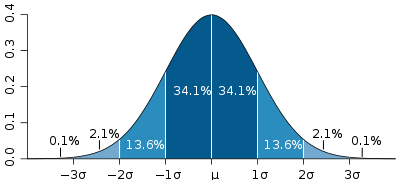
\includegraphics[scale=0.85]{regra-dos-3-sigma.png}
\label{figura:regra_3_sigmas}
\end{figure}

Após a padronização das características, a primeira tarefa é gerar o conjunto de regras baseadas nos vetores de características. A primeira etapa desse processo do conjunto de regras é definir os conjuntos fuzzy para modelar nossas variáveis de entrada e de saída;  A segunda etapa é a geração de regras fuzzy da combinação das variáveis de entrada e saída das características; A terceira etapa associa um grau para cada regra gerada; E a quarta etapa forma o conjunto final de regras fuzzy, eliminando regras repetidas e inconsistentes. Esse processo é conhecido como o método de Wang-Mendel para geração de regras fuzzy \cite{wang1992generating}. 

\subsection{O método de Wang-Mendel}

A primeira etapa de definição dos conjuntos fuzzy consiste na divisão dos dados de entrada e saída em regiões fuzzy. Nós escolhemos os conjuntos fuzzy triangulares para o mapeamento dos dados. Para os dados de saída, nós utilizamos dois conjuntos fuzzy $Positivo (P)$ e $Negativo (N)$, de mesmo tamanho, já que nossa tarefa principal é classificar o sentimento geral dos documentos em positivo ou negativo. A figura \ref{fig:conjuntos_fuzzy_saida} mostra como ficou a divisão da saída \cite{wang1992generating}. 

\begin{figure}[h]
\caption{Divisão da saída em 2 conjuntos fuzzy}
\centering
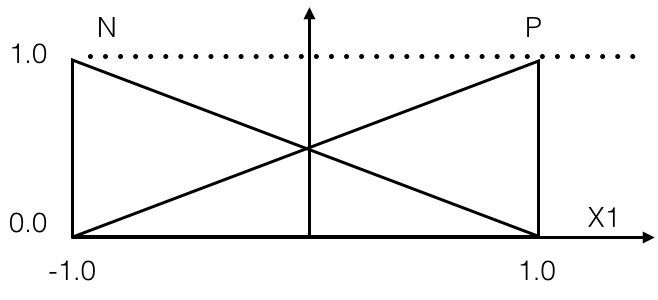
\includegraphics[scale=0.45]{conjuntos_fuzzy_saida.png}
\label{figura:conjuntos_fuzzy_saida}
\end{figure}

Para os dados de entrada, nossa primeira abordagem foi dividir igualmente, de maneira automática,os dados em $2N + 1$ \cite{wang1992generating} conjuntos fuzzy, para $N$ igual a 2, resultando em cinco regiões fuzzy: $Muito Baixo (MB)$, $Baixo (B)$, $Medio (M)$, $Alto (A)$ e $Muito Alto (MA)$. A figura \ref{figura:cinco_conjuntos_fuzzy} ilustra essa primeira abordagem.

\begin{figure}[h]
\caption{Divisão das características de entrada em 5 conjuntos fuzzy}
\centering
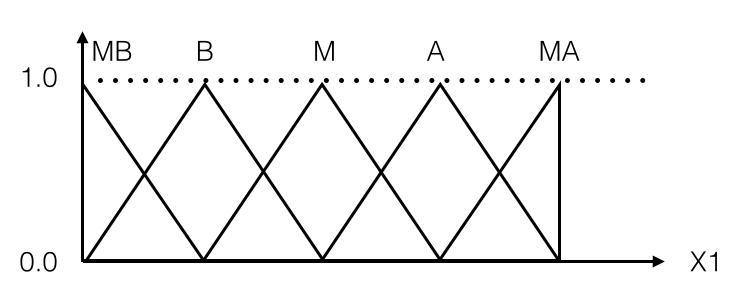
\includegraphics[scale=0.45]{cinco_conjuntos_fuzzy.png}
\label{figura:cinco_conjuntos_fuzzy}
\end{figure}

O uso de mais conjuntos fuzzy para dividir as regiões das características faz com que o mapeamento dos dados seja mais granular, possibilitando classificar casos mais específicos. Todavia, os dados das características se sobrepõem bastante, anulando esse efeito da quantidade maior de regiões fuzzy. Assim, decidimos diminuir a quantidade de regiões fuzzy, diminuindo a complexidade das regras a serem geradas e aumentando a performance da classificação. As regiões fuzzy que restaram foram $Baixo (B)$, $Medio (M)$ e $Alto (A)$, como mostra a figura \ref{figura:tres_conjuntos_fuzzy}.

\begin{figure}[h]
\caption{Divisão das características de entrada em 3 conjuntos fuzzy}
\centering
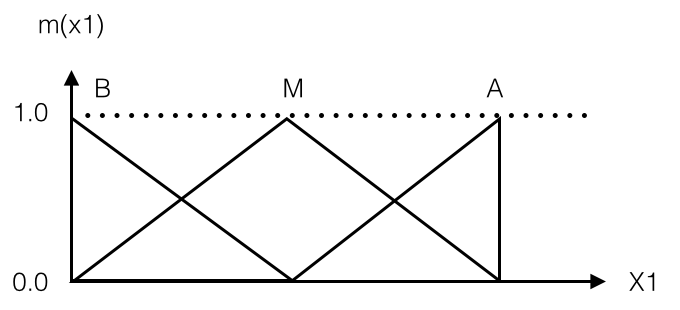
\includegraphics[scale=0.45]{tres_conjuntos_fuzzy.png}
\label{figura:tres_conjuntos_fuzzy}
\end{figure}

Mais uma vez, em nossos experimentos, a natureza de sobreposição dos dados das características se mostrou evidente com o uso do conjunto fuzzy $Medio$. A figura \ref{fig:distribuicao_dados_sobreposicao} mostra um das características extraídas na etapa anterior. É possível perceber que há significativa sobreposição dos dados na região central da distribuição onde o conjunto fuzzy $Medio$ tem maior grau de pertinência. Daí, manter o conjunto $Medio$ sob estas condições resultaria em regras que classificariam erroneamente muitos dados como médios. Assim, nós decidimos reduzir novamente a quantidade de conjuntos fuzzy para 2, $Baixo (B)$ e $Alto (A)$, como mostra a figura \ref{fig:conjuntos_fuzzy_entrada_final}. 

\begin{figure}[h]
\caption{Distribuição dos dados de uma das características da base de dados}
\centering
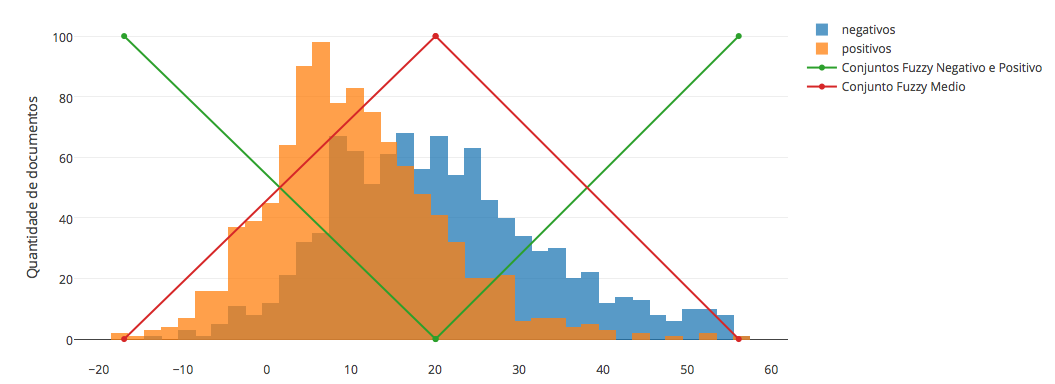
\includegraphics[scale=0.45]{distribuicao_dados_sobreposicao.png}
\label{figura:distribuicao_dados_sobreposicao}
\end{figure}

\begin{figure}[h]
\caption{Divisão das características de entrada em 2 conjuntos fuzzy}
\centering
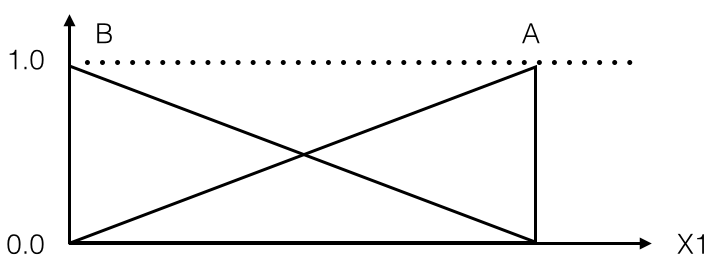
\includegraphics[scale=0.45]{conjuntos_fuzzy_entrada_final.png}
\label{figura:conjuntos_fuzzy_entrada_final}
\end{figure}

Uma vez definidas as regiões fuzzy (ou conjuntos fuzzy) dos dados de entrada e saída, a próxima tarefa é a criação do conjunto de regras baseadas nas características. Nosso conjunto de características pode ser representado da seguinte forma:

\begin{equation}
( x_1^1, x_2^1, ... , x_n^1, y^1), ( x_1^2, x_2^2, ... , x_n^2, y^2), ...
\label{eq:repr_feat}
\end{equation}

onde, $x_1^k, x_2^k, ... , x_n^k$ são os vetores de características e $y^k$ é a polaridade, positiva ou negativa, final de um documento. Para gerar regras fuzzy a partir das  características, precisamos determinar os graus de pertinência de cada característica $x_i^k$ e $y^k$ para cada conjunto fuzzy que definimos anteriormente. Por exemplo, é preciso saber qual o grau de pertinência de $x_1^1$ para o conjunto $Alto$ e para o conjunto $Baixo$, assim como para $x_1^2$ e o grau de pertinência de $y^1$ e $y^2$ para os conjuntos $Positivo$ e $Negativo$. Em seguida, associa-se cada $x_i^k$ e $y^k$ ao conjunto fuzzy com maior grau de pertinência resultante (se $x_1^1$ teve maior grau de pertinência no conjunto $Baixo$, ele será associado a essa região, e assim sucessivamente). Assim, podemos definir a criação de uma regra fuzzy da seguinte forma:

\begin{equation}
\begin{split}
( x_1^k, x_2^k, ... , x_n^k, y^k) => [x_1^k (Pol(x_1^k) \, em \, CFI_n, max), \, ... \, , x_n^k (Pol(x_2^k) \, em \, CFI_m, max); \\
y^k(Pol(y^k) \, em \, CFS_n, max)] => Regra \, k: \\ IF \, x_1^k \, is \, CFI_n \, and \, ... \, x_n^k \, is \, CFI_m, \, THEN \, y^k \, is \, CFS_n
\label{eq:repr_fuzzy_rule}
\end{split}
\end{equation}

onde $(Pol(x_1^k) \, em \, CFI_n, max)$ é o grau máximo de pertinência alcançado por $x_1^k$ em um dos conjuntos fuzzy de entrada $CFI_n$ e $(Pol(y^k) \, em \, CFS_n, max)$ é o grau máximo de pertinência alcançado por $y^k$ um um dos conjuntos fuzzy de saída $CFS_n$. As regras geradas são do tipo "AND", que são regras em que as condições antecedentes, a parte do IF, tem de, simultaneamente ocorrer em ordem para que o conseqüente, a parte THEN, aconteça. 

A tarefa de geração de regras cria uma regra para cada vetor de característica. Devido a grande quantidade de vetores de características, é muito provável que regras conflitantes tenham sido geradas, como regras com mesmo antecedente, mas com conseqüente diferente. Uma maneira proposta pelo método de Wang-Mendel é associar um grau a cada regra e descartando a regra conflitante com menor grau. Além de eliminar regras contraditórias, esse método também reduz a quantidade de regras a serem usadas na classificação. A seguinte estratégia é utilizada para associar um grau $D(regra)$ a cada regra: 

\begin{equation}
D(regra) = m_{CFI_n}(x_1) \cdot m_{CFI_m}(x_2) \cdot m_{CFI_o}(x_n) \cdot ... \cdot m_{CFS_n}(y)
\label{eq:grau_regra}
\end{equation}

onde $m_{CFI_o}(x_n)$, por exemplo, é o grau de pertinência de $x_n$ no conjunto fuzzy $CFI_o$. Por exemplo, considere uma regra com duas características: "IF $x_1$ is Alto and $x_2$ is Alto, THEN $y$ is Positivo". O grau dessa regra, utilizando a estratégia \ref{eq:grau_regra}, é obtido assim:  $D(regra) = m_{Alto}(x_1) \cdot m_{Alto}(x_2) \cdot m_{Positivo}(y)$. Depois de eliminadas as regras conflitantes, as regras finais constituem o conjunto de regras fuzzy baseado nas características dos documentos. Com esse conjunto de regras é possível classificar os documentos da base de dados.

\subsection{Classificação}

O conjunto gerado de regras fuzzy é usado, agora, por um mecanismo de inferência fuzzy para determinar a polaridade final dos documentos da base. Nós utilizamos dois mecanismos para fins de comparação que foram Método Geral do Raciocínio Fuzzy (MGRF) e o Método Clássico do Raciocínio Fuzzy (MCRF) \cite{cordon1999proposal}.
Ambos mecanismos tem processos bastante similares e somente diferente na etapa de decisão na classificação. O mecanismo comum a ambos é: cada vetor de característica é avaliado por todas as regras fuzzy do conjunto gerado e um grau de compatibilidade \ref{eq:compat_regra} é produzido para cada regra. 

\begin{equation}
D(regra) = m_{CFI_n}(x_1) \cdot m_{CFI_m}(x_2) \cdot m_{CFI_o}(x_3) \cdot ...\cdot m_{CFI_p}(x_n)
\label{eq:compat_regra}
\end{equation}

O MCRF escolhe a regra com o máximo grau de compatibilidade para um dado vetor de característica e classifica o documento relacionado com a classe da regra escolhida. Por outro lado, o MGRF considera o máximo grau médio de compatibilidade entre as duas classes possíveis, positivo e negativo. Em outras palavras, o MGRF calcula a média dos graus de compatibilidade das regras que tem o consequente com a classe positiva e negativa e classifica o documento com a classe de maior média resultante. 

\section{Avaliação}

